% !TeX program = xelatex
% !TeX encoding = UTF-8
\documentclass[10pt,a4paper,fontset=fandol]{ctexart}
\usepackage[top=1.20cm,bottom=1.20cm,left=1.40cm,right=1.40cm]{geometry}
\usepackage{graphicx}
\usepackage{xcolor}
\usepackage{enumitem}
\usepackage{tabularx}
\usepackage[hidelinks]{hyperref}
\usepackage{atbegshi}
\pagestyle{empty}
\setlength{\parindent}{0pt}
\setlength{\parskip}{0pt}
\setlength{\emergencystretch}{2em}
\linespread{1}
\definecolor{accent}{HTML}{234A66}
\definecolor{muted}{HTML}{4D5963}
\definecolor{ruleColor}{HTML}{B8C7D2}
\setmainfont{texgyreheros-regular.otf}[BoldFont=texgyreheros-bold.otf,ItalicFont=texgyreheros-italic.otf]
\setCJKmainfont[BoldFont=FandolHei-Bold.otf]{FandolSong-Regular.otf}
\setCJKsansfont[BoldFont=FandolHei-Bold.otf]{FandolHei-Regular.otf}
% Section rules occupy a separate paragraph to prevent title overlap.
\newcommand{\cvsection}[1]{%
  \par\vspace{6pt}%
  {\sffamily\bfseries\fontsize{12.5}{15}\selectfont\color{accent}#1\par}%
  \vspace{2pt}{\color{ruleColor}\hrule height 0.5pt}\vspace{4pt}%
}
\newcommand{\entrytitle}[2]{%
  \par\noindent\begin{tabularx}{\linewidth}{@{}Xr@{}}%
    {\bfseries #1} & {\small\color{muted}#2}%
  \end{tabularx}\par\vspace{1pt}%
}
\newcommand{\tech}[1]{{\fontsize{9.3}{12}\selectfont\color{muted}#1\par}\vspace{1pt}}
\setlist[itemize]{label=\textbullet,leftmargin=1.15em,labelsep=0.45em,
  itemsep=2pt,topsep=2pt,parsep=0pt,partopsep=0pt}
% Fail compilation if future edits spill onto a second page.
\newcount\cvpages
\AtBeginShipout{\global\advance\cvpages by 1
  \ifnum\cvpages>1\PackageError{cv}{Resume exceeds one page}{Shorten the content or adjust spacing.}\fi}
\begin{document}
\fontsize{10.5}{14.2}\selectfont
\noindent\begin{minipage}[c]{0.83\textwidth}
  {\sffamily\bfseries\fontsize{23}{27}\selectfont 李昕潼}\par\vspace{7pt}
  电话：18543740228\quad\textcolor{ruleColor}{|}\quad
  \href{mailto:xintong.li@u.nus.edu}{xintong.li@u.nus.edu}
\end{minipage}\hfill%
\begin{minipage}[c]{0.14\textwidth}
  \raggedleft
  \IfFileExists{assets/resume_photo.png}{%
    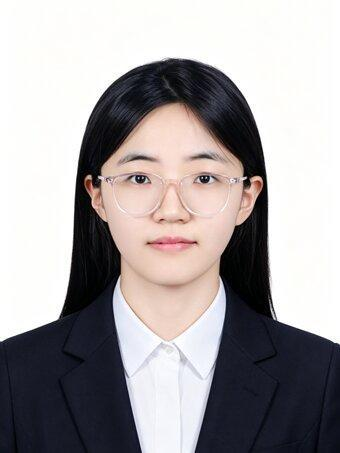
\includegraphics[width=1.85cm]{assets/resume_photo.png}%
  }{\rule{0pt}{2.46cm}}
\end{minipage}\par
\cvsection{教育背景}
\entrytitle{新加坡国立大学\quad 计算机硕士（MComp）}{2026/08 -- 至今}
\entrytitle{北京邮电大学\quad 通信工程本科}{2022/09 -- 2026/06}
均分 \textbf{90.47}；国家奖学金、大一学年一等奖学金；北京市优秀毕业生。
\cvsection{实习经历}
\entrytitle{快手\quad AI Agent 开发工程师}{2026/05 -- 2026/07}
\tech{TypeScript / LangGraph / OpenCode / Tool Calling / Multi-Agent / React / Node.js}
参与 Code、Design 与 Prototype Agent 研发，将 Figma 设计稿自动转换为跨端代码与交互原型。
\begin{itemize}
  \item \textbf{独立开发 Figma-to-Prototype 流程}：解析节点树，将布局、组件与样式转为结构化上下文，结合 Agent 推理生成可运行前端原型。
  \item \textbf{优化 Design-to-Code 链路}：基于 OpenCode 串联设计理解、代码生成与工程写入，结合 SVG/PNG 资源 CDN 化处理，支持 RN、KRN、Vue；通过工具调用自动创建文件并写入代码。
  \item \textbf{扩展多页面与交互生成}：设计页面级上下文管理和跨页面交互建模，支持多设计稿联合生成；抽取跳转关系与交互配置，生成路由、页面切换及动效逻辑。
\end{itemize}
\cvsection{项目经历}
\entrytitle{基于大模型智能体的网络故障根因定位系统}{2025/12 -- 2026/03}
\tech{Python / Qwen2.5-7B-Instruct / PEFT / LoRA / GRPO / LangChain / ReAct / RAG}
\begin{itemize}
  \item \textbf{构建 2,400 条 SFT 样本}：基于 TeleLogs 设计两阶段蒸馏流程，以排除、矛盾、规则和统计策略生成推理轨迹，再由教师模型整合、压缩与标准化。
  \item \textbf{模型训练与 Agent 诊断}：使用 PEFT/LoRA 微调 Qwen2.5-7B-Instruct，结合 GRPO 优化根因判别；基于 LangChain/ReAct 封装表格解析、故障区间、小区几何及干扰分析工具，结合规则知识库与 RAG 完成多步诊断。
  \item \textbf{实验结果}：Pass@1 由基础模型的 12.04\% 提升至微调后的 53.59\%，引入 Agent 后达到 \textbf{76.50\%}；Pass@4 对应由 12.50\% 提升至 54.86\% 和 \textbf{78.36\%}。
\end{itemize}
\vspace{3pt}
\entrytitle{CADDesigner：基于通用智能体的 CAD 模型设计系统}{2025/06 -- 2025/09}
\tech{Python / LangChain / Claude Sonnet / CadQuery / PythonOCC / ReAct / Function Calling}
\begin{itemize}
  \item \textbf{设计文本/图像到 CAD 的生成闭环}：基于 LangChain 组织多步推理和工具调用，使用 Claude Sonnet 提取几何特征与约束，生成 CadQuery/PythonOCC 参数化建模代码。
  \item \textbf{实现视觉反馈迭代修复}：在 sandbox 中执行代码、构建模型并渲染标准三视图，由 Agent 评估视觉一致性；存在偏差时修正或重新生成代码，持续优化模型。
  \item \textbf{实验结果}：在 CAD-VGDrawing 上取得 IoU 0.2769、CD 0.1097、HD 0.4347，\textbf{有效模型生成成功率（SUC）100.0\%}。
\end{itemize}
\cvsection{技能特长}
\textbf{开发环境：}Linux、Shell、Git、Conda、远程 GPU 服务器。\par
\textbf{模型训练：}LoRA/QLoRA、PEFT、GRPO；数据构建、领域微调与效果评测。\par
\textbf{智能体开发：}LangGraph、LangChain、ReAct、Tool Calling、Multi-Agent、RAG。
\end{document}
